\documentclass[tikz,border=4pt]{standalone}
\usepackage{amsmath}
\usepackage{graphicx}
\usepackage{tikz}
\usetikzlibrary{calc}

% Adjust these font commands later without touching the saved positions.
\newcommand{\marTwentySixFormulaFont}{\fontsize{14}{14}\selectfont}
\newcommand{\marTwentySixNumberFont}{\fontsize{12}{12}\selectfont}

\tikzset{
  mar26 psi/.style={font=\marTwentySixFormulaFont,text=black,anchor=center,inner sep=0pt,outer sep=0pt},
  mar26 phi/.style={font=\marTwentySixFormulaFont,text=black,anchor=center,inner sep=0pt,outer sep=0pt},
  mar26 top plus/.style={font=\marTwentySixFormulaFont,text=black,anchor=center,inner sep=0pt,outer sep=0pt},
  mar26 vertical plus/.style={font=\marTwentySixFormulaFont,text=black,anchor=center,inner sep=0pt,outer sep=0pt},
  mar26 equals/.style={font=\marTwentySixFormulaFont,text=black,anchor=center,inner sep=0pt,outer sep=0pt},
  mar26 pair title/.style={font=\marTwentySixFormulaFont,text=black,anchor=center,inner sep=0pt,outer sep=0pt},
  mar26 pair focus/.style={font=\marTwentySixFormulaFont,text=black,anchor=center,inner sep=0pt,outer sep=0pt},
  mar26 pair neighbour/.style={font=\marTwentySixFormulaFont,text=black,anchor=center,inner sep=0pt,outer sep=0pt},
  mar26 number/.style={font=\marTwentySixNumberFont,text=black,anchor=center,inner sep=0pt,outer sep=0pt,text height=1.5ex,text depth=0.25ex},
  mar26 neighbour number/.style={font=\marTwentySixNumberFont,text={rgb,1:red,0.55;green,0.55;blue,0.55},anchor=center,inner sep=0pt,outer sep=0pt,text height=1.5ex,text depth=0.25ex}
}

\begin{document}
\begin{tikzpicture}
  \node[inner sep=0pt,outer sep=0pt] (img) at (0,0) {%
    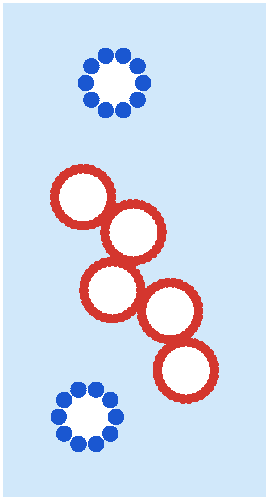
\includegraphics{mar26_visualse_coarse_fine_fig2.pdf}%
  };
  % Auto-generated from mar26_visualse_coarse_fine.m
\begin{scope}[shift={(img.south west)},
  x={($(img.south east)-(img.south west)$)},
  y={($(img.north west)-(img.south west)$)}]
  \node[mar26 number] at (0.1619538877648449, 0.6798554818311022) {1};
  \node[mar26 number] at (0.6066834154282338, 0.6957392741260747) {2};
  \node[mar26 number] at (0.4184971350243847, 0.5842675341874608) {3};
  \node[mar26 number] at (0.5353549126909776, 0.5043617882216359) {4};
  \node[mar26 number] at (0.3759643823112471, 0.3647283014616796) {5};
  \node[mar26 number] at (0.2529522764051008, 0.3042607258739254) {6};
  \node[mar26 number] at (0.8322620448149821, 0.5762082746756041) {7};
\end{scope}

\end{tikzpicture}
\end{document}
